\let\negmedspace\undefined
\let\negthickspace\undefined
\documentclass[journal]{IEEEtran}
\usepackage[a5paper, margin=10mm, onecolumn]{geometry}
%\usepackage{lmodern} % Ensure lmodern is loaded for pdflatex
\usepackage{tfrupee} % Include tfrupee package

\setlength{\headheight}{1cm} % Set the height of the header box
\setlength{\headsep}{0mm}     % Set the distance between the header box and the top of the text

\usepackage{gvv-book}
\usepackage{gvv}
\usepackage{cite}
\usepackage{amsmath,amssymb,amsfonts,amsthm}
\usepackage{algorithmic}
\usepackage{graphicx}
\usepackage{textcomp}
\usepackage{xcolor}
\usepackage{txfonts}
\usepackage{listings}
\usepackage{enumitem}
\usepackage{mathtools}
\usepackage{gensymb}
\usepackage{comment}
\usepackage[breaklinks=true]{hyperref}
\usepackage{tkz-euclide} 
\usepackage{listings}
% \usepackage{gvv}                                        
\def\inputGnumericTable{}                                 
\usepackage[latin1]{inputenc}                                
\usepackage{color}                                            
\usepackage{array}                                            
\usepackage{longtable}                                       
\usepackage{calc}                                             
\usepackage{multirow}                                         
\usepackage{hhline}                                           
\usepackage{ifthen}                                           
\usepackage{lscape}

\begin{document}

\bibliographystyle{IEEEtran}
\vspace{3cm}

\title{4.10.17}
\author{EE25BTECH11015 - Bhoomika V}
% \maketitle
% \newpage
% \bigskip
{\let\newpage\relax\maketitle}

\renewcommand{\thefigure}{\theenumi}
\renewcommand{\thetable}{\theenumi}
\setlength{\intextsep}{10pt} % Space between text and floats


\numberwithin{equation}{enumi}
\numberwithin{figure}{enumi}
\renewcommand{\thetable}{\theenumi}
\parindent 0px 
{Question :-} \\ 
Compute the area bounded by the lines $x + 2y = 2$, $y - x = 1$, and $2x + y = 7$.
\\ \\ 
\solution \\
Equations of the lines \\
\[
L_1: x + 2y = 2, \quad 
L_2: y - x = 1, \quad
L_3: 2x + y = 7
\]


 Finding intersection points using RREF \\

Intersection of $L_1$ and $L_2$:
\[
\begin{cases}
x + 2y = 2 \\
-x + y = 1
\end{cases}
\]
\[
\left[\begin{array}{cc|c}
1 & 2 & 2 \\
-1 & 1 & 1
\end{array}\right]
\;\;\xrightarrow{\text{RREF}}\;\;
\left[\begin{array}{cc|c}
1 & 0 & 0 \\
0 & 1 & 1
\end{array}\right]
\]
\[
A= (0,1)
\]

Intersection of $L_2$ and $L_3$:
\[
\begin{cases}
-x + y = 1 \\
2x + y = 7
\end{cases}
\]
\[
\left[\begin{array}{cc|c}
-1 & 1 & 1 \\
2 & 1 & 7
\end{array}\right]
\;\;\xrightarrow{\text{RREF}}\;\;
\left[\begin{array}{cc|c}
1 & 0 & 2 \\
0 & 1 & 3
\end{array}\right]
\]
\[
B = (2,3)
\]

Intersection of $L_1$ and $L_3$:
\[
\begin{cases}
x + 2y = 2 \\
2x + y = 7
\end{cases}
\]
\[
\left[\begin{array}{cc|c}
1 & 2 & 2 \\
2 & 1 & 7
\end{array}\right]
\;\;\xrightarrow{\text{RREF}}\;\;
\left[\begin{array}{cc|c}
1 & 0 & 4 \\
0 & 1 & -1
\end{array}\right]
\]
\[
C = (4,-1)
\]


Area of the triangle

\[
\Delta = \tfrac{1}{2} \left| (\vec{A}-\vec{B}) \times (\vec{B}-\vec{C}) \right|
\]

Compute:
\[
\vec{A} - \vec{B} = \begin{bmatrix} -2 \\ -2 \end{bmatrix}, \quad
\vec{B} - \vec{C} = \begin{bmatrix} -2 \\ 4 \end{bmatrix}
\]

\[
(\vec{A}-\vec{B}) \times (\vec{B}-\vec{C}) =
\begin{vmatrix}
-2 & -2 \\
-2 & 4
\end{vmatrix}
= (-2)(4) - (-2)(-2) = -12
\]

\[
\Delta = \tfrac{1}{2} | -12 | = 6
\]



Final Answer:
\[
\text{Area} = 6
\]
\begin{figure}[H]
\begin{center}
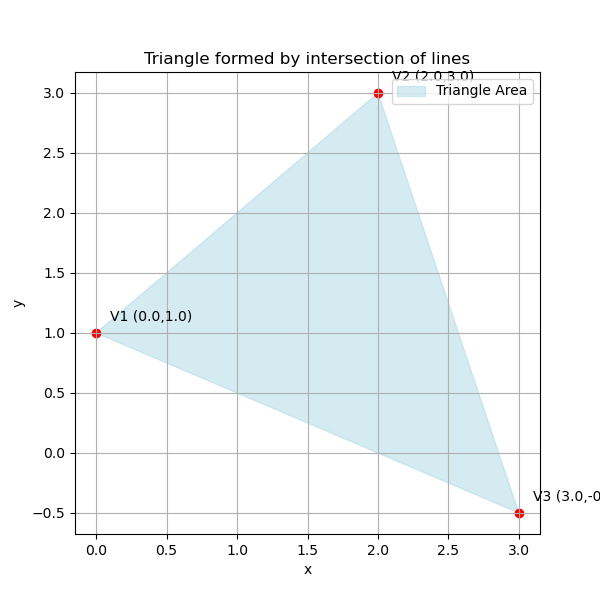
\includegraphics[width=0.6\columnwidth]{Figs/Fig1.png}
\end{center}
\caption{}
\label{fig:Fig.1}
\end{figure}


\end{document}
